% (find-LATEX "2021-2-C3-tipos.tex")
% (defun c () (interactive) (find-LATEXsh "lualatex -record 2021-2-C3-tipos.tex" :end))
% (defun C () (interactive) (find-LATEXsh "lualatex 2021-2-C3-tipos.tex" "Success!!!"))
% (defun D () (interactive) (find-pdf-page      "~/LATEX/2021-2-C3-tipos.pdf"))
% (defun d () (interactive) (find-pdftools-page "~/LATEX/2021-2-C3-tipos.pdf"))
% (defun e () (interactive) (find-LATEX "2021-2-C3-tipos.tex"))
% (defun o () (interactive) (find-LATEX "2021-1-C3-tipos.tex"))
% (defun u () (interactive) (find-latex-upload-links "2021-2-C3-tipos"))
% (defun v () (interactive) (find-2a '(e) '(d)))
% (defun d0 () (interactive) (find-ebuffer "2021-2-C3-tipos.pdf"))
% (defun cv () (interactive) (C) (ee-kill-this-buffer) (v) (g))
%          (code-eec-LATEX "2021-2-C3-tipos")
% (find-pdf-page   "~/LATEX/2021-2-C3-tipos.pdf")
% (find-sh0 "cp -v  ~/LATEX/2021-2-C3-tipos.pdf /tmp/")
% (find-sh0 "cp -v  ~/LATEX/2021-2-C3-tipos.pdf /tmp/pen/")
%     (find-xournalpp "/tmp/2021-2-C3-tipos.pdf")
%   file:///home/edrx/LATEX/2021-2-C3-tipos.pdf
%               file:///tmp/2021-2-C3-tipos.pdf
%           file:///tmp/pen/2021-2-C3-tipos.pdf
% http://angg.twu.net/LATEX/2021-2-C3-tipos.pdf
% (find-LATEX "2019.mk")
% (find-CN-aula-links "2021-2-C3-tipos" "3" "c3m212types" "c3ty")

% «.defs»		(to "defs")
% «.title»		(to "title")
% «.tipos»		(to "tipos")
% «.exercicio-1»	(to "exercicio-1")
% «.exercicio-2»	(to "exercicio-2")
% «.exercicio-3»	(to "exercicio-3")
% «.exercicio-4»	(to "exercicio-4")
% «.exercicio-5»	(to "exercicio-5")
% «.intro-nf»		(to "intro-nf")
% «.primeiro-exemplo»	(to "primeiro-exemplo")
% «.material-de-2021.1»	(to "material-de-2021.1")
%
% «.djvuize»		(to "djvuize")
% «.elisp»		(to "elisp")



% <videos>
% Video (not yet):
% (find-ssr-links     "c3m212types" "2021-2-C3-tipos")
% (code-eevvideo      "c3m212types" "2021-2-C3-tipos")
% (code-eevlinksvideo "c3m212types" "2021-2-C3-tipos")
% (find-c3m212typesvideo "0:00")

\documentclass[oneside,12pt]{article}
\usepackage[colorlinks,citecolor=DarkRed,urlcolor=DarkRed]{hyperref} % (find-es "tex" "hyperref")
\usepackage{amsmath}
\usepackage{amsfonts}
\usepackage{amssymb}
\usepackage{pict2e}
\usepackage[x11names,svgnames]{xcolor} % (find-es "tex" "xcolor")
\usepackage{colorweb}                  % (find-es "tex" "colorweb")
%\usepackage{tikz}
%
% (find-dn6 "preamble6.lua" "preamble0")
%\usepackage{proof}   % For derivation trees ("%:" lines)
%\input diagxy        % For 2D diagrams ("%D" lines)
%\xyoption{curve}     % For the ".curve=" feature in 2D diagrams
%
\usepackage{edrx21}               % (find-LATEX "edrx21.sty")
\input edrxaccents.tex            % (find-LATEX "edrxaccents.tex")
\input edrx21chars.tex            % (find-LATEX "edrx21chars.tex")
\input edrxheadfoot.tex           % (find-LATEX "edrxheadfoot.tex")
\input edrxgac2.tex               % (find-LATEX "edrxgac2.tex")
%
%\usepackage[backend=biber,
%   style=alphabetic]{biblatex}            % (find-es "tex" "biber")
%\addbibresource{catsem-slides.bib}        % (find-LATEX "catsem-slides.bib")
%
% (find-es "tex" "geometry")
\usepackage[a6paper, landscape,
            top=1.5cm, bottom=.25cm, left=1cm, right=1cm, includefoot
           ]{geometry}
%
\begin{document}

%\catcode`\^^J=10
%\directlua{dofile "dednat6load.lua"}  % (find-LATEX "dednat6load.lua")

% %L dofile "edrxtikz.lua"  -- (find-LATEX "edrxtikz.lua")
% %L dofile "edrxpict.lua"  -- (find-LATEX "edrxpict.lua")
% \pu

% «defs»  (to ".defs")
% (find-LATEX "edrx21defs.tex" "colors")
% (find-LATEX "edrx21.sty")

\def\drafturl{http://angg.twu.net/LATEX/2021-2-C3.pdf}
\def\drafturl{http://angg.twu.net/2021.2-C3.html}
\def\draftfooter{\tiny \href{\drafturl}{\jobname{}} \ColorBrown{\shorttoday{} \hours}}

\def\rq{\ColorRed{?}}
\def\undq#1{\underbrace{#1}_{\rq}}




%  _____ _ _   _                               
% |_   _(_) |_| | ___   _ __   __ _  __ _  ___ 
%   | | | | __| |/ _ \ | '_ \ / _` |/ _` |/ _ \
%   | | | | |_| |  __/ | |_) | (_| | (_| |  __/
%   |_| |_|\__|_|\___| | .__/ \__,_|\__, |\___|
%                      |_|          |___/      
%
% «title»  (to ".title")
% (c3m212typesp 1 "title")
% (c3m212typesa   "title")

\thispagestyle{empty}

\begin{center}

\vspace*{1.2cm}

{\bf \Large Cálculo 3 - 2021.2}

\bsk

Aula 9: tipos

\bsk

Eduardo Ochs - RCN/PURO/UFF

\url{http://angg.twu.net/2021.2-C3.html}

\end{center}

\newpage

% «tipos»  (to ".tipos")
% (c3m212typesp 2 "tipos")
% (c3m212typesa   "tipos")
% (c3m211vlp 3 "tipos")
% (c3m211vla   "tipos")
% (find-LATEXgrep "grep --color=auto -nH --null -e tipos 2020-2-C3*.tex")
% (c3m202rcadeia1p 8 "tipos")
% (c3m202rcadeia1a   "tipos")

{\bf Tipos}

\ssk

\scalebox{0.6}{\def\colwidth{8cm}\firstcol{

{\bf TUDO} que nós vamos fazer em Cálculo 3 pode ser {\sl visualizado}
e {\sl tipado}. Você já viu um pouco de tipos em {\tt C} e em Física;
em Física os ``tipos'' são parcialmente determinados pelas unidades
--- metros são distância, segundos são tempo, metros/segundo é uma
unidade de velocidade, e assim por diante... em {\tt C} um {\tt char},
um {\tt int}, um {\tt float} e um {\tt (void *)} são coisas bem
diferentes.

\ssk

Obs: o jeito como nós vamos usar tipos em Cálculo 3 vai ser bastante
improvisado. Se você googlar por ``Type Theory'' você vai encontrar
montes de referências a teorias de tipos que podem ser totalmente
formalizadas, mas os tipos que nós vamos usar em C3 são muito mais
``intuitivos'' do que ``formais''.

\ssk
}\anothercol{

% (find-bortolossi5page (+ -162 164) "5.2. Definições e exemplos")
% (find-bortolossi5page (+ -162 165)   "Fig. 5.2: Interpretação geométrica")

Dê uma olhada nas páginas 164 a 166 do capítulo 5 do Bortolossi. Todas
as expressões que aparecem lá podem ser ``tipadas'' e interpretadas
como posições no eixo $x$ (ou no eixo $y$, ou no eixo $y$), ou como
distâncias no eixo $x$ (ou no eixo $y$, ou $z$), ou como {\sl
  inclinações}... vamos ver os detalhes disto aos poucos.

\ssk

Nos próximos exercícios você vai tentar ``tipar'' cada subexpressão
deles. Escreva os seus tipos nos lugares em que eu pus as `$\rq$'s.
Use português, improvise o quanto precisar, invente abreviações -- mas
tente encontrar as melhores abreviações possíveis -- e compare o seu
modo de escrever os tipos com os dos seus colegas. Lembre que aqui nós
estamos tentando fazer explicitamente, num diagrama, algo que os
livros fazem em poucas frases de texto fingindo que é algo óbvio.

Se você tiver dificuldade de fazer o caso geral faça um caso
particular primeiro.


}}

\newpage

% «exercicio-1»  (to ".exercicio-1")
% (c3m212typesp 3 "exercicio-1")
% (c3m212typesa   "exercicio-1")
% (c3m211vlp 5 "exercicio-1")
% (c3m211vla   "exercicio-1")
% (c3m202rcadeia1p 32 "tipos-de-novo")
% (c3m202rcadeia1a    "tipos-de-novo")

{\bf Exercício 1}

Digamos que $f(x)=x^2$ e que $y=f(x)$. 

Se você tiver dificuldade de pensar no caso geral

faça $x_0=1$ e $Δx=0.1$.

$$\undq{
  \undq{(\undq{\undq{f}(\undq{\undq{x_0} + \undq{Δx}})}
        - \undq{\undq{f}(\undq{x_0})})} / \undq{Δx}
  }
$$


\newpage

% «exercicio-2»  (to ".exercicio-2")
% (c3m212typesp 4 "exercicio-2")
% (c3m212typesa   "exercicio-2")
% (c3m211vlp 6 "exercicio-2")
% (c3m211vla   "exercicio-2")

{\bf Exercício 2}

Digamos que $f(t)=\cos t$, $g(t)=\sen t$, e $P(t)=(f(t),g(t))$. 

Se você tiver dificuldade de pensar no caso geral

faça $t_0=\fracπ2$ e $Δt=0.1$.

$$\undq{
  \undq{(\undq{\undq{P}(\undq{\undq{t_0} + \undq{Δt}})}
        - \undq{\undq{P}(\undq{t_0})})} / \undq{Δt}
  }
$$

\newpage

% «exercicio-3»  (to ".exercicio-3")
% (c3m212typesp 5 "exercicio-3")
% (c3m212typesa   "exercicio-3")
% (c3m211vlp 7 "exercicio-3")
% (c3m211vla   "exercicio-3")

{\bf Exercício 3}

Digamos que $f(t)=\cos t$, $g(t)=\sen t$, e $P(t)=(f(t),g(t))$. 

Se você tiver dificuldade de pensar no caso geral

faça $t_0=\fracπ2$ e $Δt=0.1$.
%
$$\undq{\undq{P}(\undq{\undq{t_0} + \undq{Δt}})}
  =
  \undq{
    ( \undq{\undq{f}(\undq{\undq{t_0} + \undq{Δt}})},
      \undq{\undq{g}(\undq{\undq{t_0} + \undq{Δt}})} )
  }
$$

\newpage

% «exercicio-4»  (to ".exercicio-4")
% (c3m212typesp 6 "exercicio-4")
% (c3m212typesa   "exercicio-4")
% (c3m211vlp 8 "exercicio-4")
% (c3m211vla   "exercicio-4")
% (find-bortolossi6page (+ -186 197) "6.2 O vetor tangente a uma curva parametrizada")
% (find-bortolossi6page (+ -186 198)   "mas este vetor limite pode ser calculado")
% (find-bortolossi6page (+ -186 199)   "limite de vetores secantes")

Agora nós vamos começar a ver como decifrar definições

como a das páginas 197--198 do capítulo 6 do Bortolossi.

Ele faz tudo de um jeito bem geral, e ele usa $\R^m$ ao invés

de $\R^2$ ou $\R^3$.

\bsk

{\bf Exercício 4}

Reescreva a conta grande no meio da página 198 do Bortolossi

substituindo $t_0$ por $\fracπ2$, $h_j$ por $ε$,
$x_1(t)$ por $\cos t$, $x_2(t)$ por $\sen t$,

e $m$ por 2. Obs: os `$\ldots$' vão sumir.

\newpage

O livro do Bortolossi tem essa figura daqui na página 199:
%
% (find-latexscan-links "C3" "20210625_bortolossi_p199")
% (find-xpdf-page "~/LATEX/2021-1-C3/20210625_bortolossi_p199.pdf")
$$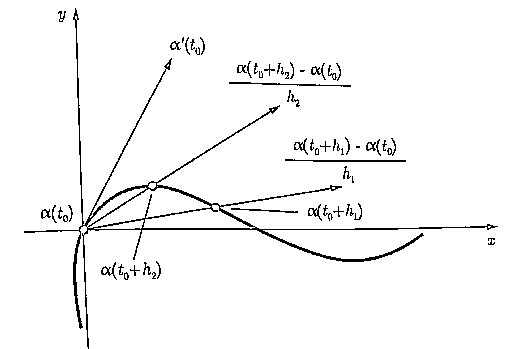
\includegraphics[height=4.5cm]{2021-1-C3/20210625_bortolossi_p199.pdf}$$

Isso é um desenho de vetor velocidade como limite de retas secantes
num caso geral -- o Bortolossi não nos diz quem são $α:\R→\R^2$, nem
$t_0$, nem a sequência $(h_1, h_2, h_3, \ldots)$, e isso sugere que
essa figura vai valer pra quaisquer $α$, $t_0$ e $(h_1, h_2, \ldots)$,
com as devidas adaptações...

\newpage

% «exercicio-5»  (to ".exercicio-5")
% (c3m212typesp 8 "exercicio-5")
% (c3m212typesa   "exercicio-5")
% (c3m211vlp 10 "exercicio-5")
% (c3m211vla    "exercicio-5")

{\bf Exercício 5}

Aqui nós vamos tentar fazer uma figura parecida com

a do caso anterior, mas com $α(t) = (\cos t, \sen t)$, $t_0=\fracπ2$,

$h_0 = \fracπ2$, $0 < \ldots < h_3 < h_2 < h_1 < h_0$, $\lim_{j→∞} h_j = 0$.

Comece com esta figura aqui,
%
% (find-latexscan-links "C3" "20210625_bortolossi_p199_hack")
% (find-xpdf-page "~/LATEX/2021-1-C3/20210625_bortolossi_p199_hack.pdf")
$$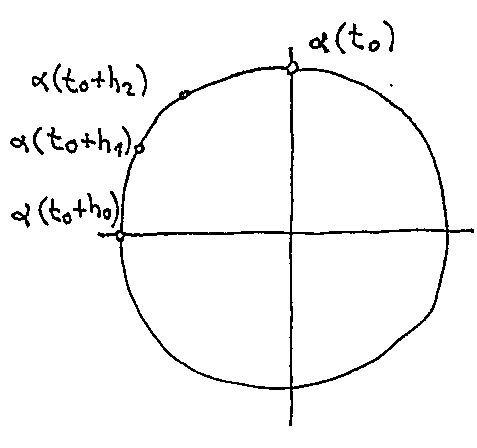
\includegraphics[height=3cm]{2021-1-C3/20210625_bortolossi_p199_hack.pdf}$$

e encontre valores razoáveis para $h_1$, $h_2$ e $h_3$ que te

permitam completar o desenho no olhômetro fazendo

as contas de cabeça com aproximações bem grosseiras.



\newpage

%  _   _ _____ 
% | \ | |  ___|
% |  \| | |_   
% | |\  |  _|  
% |_| \_|_|    
%              
% «intro-nf»  (to ".intro-nf")
% (c3m212typesp 9 "intro-nf")
% (c3m212typesa   "intro-nf")

{\bf Introdução à ``notação de físicos''}

\ssk

Nós vamos aprender a usar duas convenções de notação matemática no
curso -- ou, pra encurtar, duas ``notações''. O Bortolossi usa uma
notação muito mais precisa, que eu vou chamar de ``notação de
matemáticos'', e o Silvanus Thompson usa uma notação mais intuitiva
mas bem mais difícil de formalizar, que eu vou chamar de ``notação de
físicos''.

\ssk

Na ``notação de físicos'' muitos símbolos vão ser {\sl abreviações} e
as regras pra expandir essas abreviações vão depender do contexto. Vão
existir algumas convenções pra expandir essas abreviações que vão ser
seguidas {\sl quase} sempre, mas vão existir muitas exceções -- e
muitos casos ambíguos...

\newpage

% «primeiro-exemplo»  (to ".primeiro-exemplo")
% (c3m212typesp 10 "primeiro-exemplo")
% (c3m212typesa    "primeiro-exemplo")
% (c3m211nfp 6 "primeiro-exemplo")
% (c3m211nfa   "primeiro-exemplo")

{\bf Um primeiro exemplo}

Digamos que $y=\sqrt{x}$.

Podemos considerar que $x$ e $y$ ``variam juntos'',

``obedecendo certas restrições''. O conjunto dos pontos $(x,y)$

que obedecem essas restrições é $\setofxyst{y = \sqrt{x}}$

e o gráfico é:
%
% (find-latexscan-links "C3" "20210804_sqrt")
% (find-xpdf-page "~/LATEX/2021-1-C3/20210804_sqrt.pdf")
$$\myvcenter{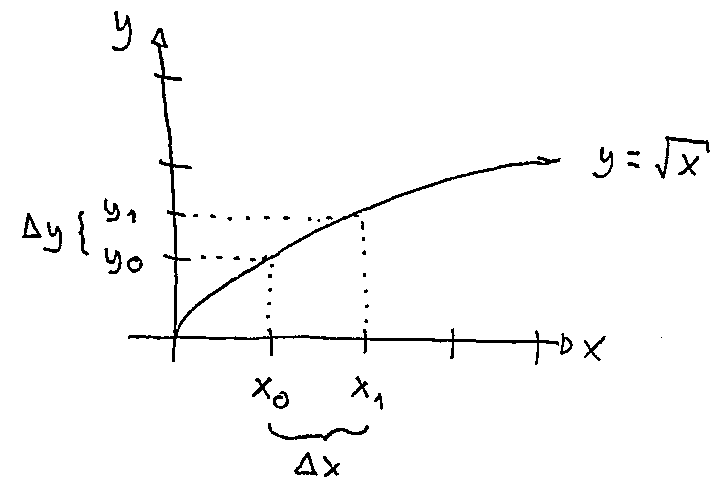
\includegraphics[height=4cm]{2021-1-C3/20210804_sqrt.pdf}}
  \qquad
  \begin{array}{rcl}
    x_0,x_1&∈&\R \\ 
    y_0 &=& \sqrt{x_0} \\ 
    y_1 &=& \sqrt{x_1} \\ 
    Δx &=& x_1 - x_0 \\
    Δy &=& y_1 - y_0 \\
    \\
  \end{array}
$$


\newpage

%  __  __       _     ____   ___ ____  _   _ 
% |  \/  | __ _| |_  |___ \ / _ \___ \/ | / |
% | |\/| |/ _` | __|   __) | | | |__) | | | |
% | |  | | (_| | |_   / __/| |_| / __/| |_| |
% |_|  |_|\__,_|\__| |_____|\___/_____|_(_)_|
%                                            
% «material-de-2021.1»  (to ".material-de-2021.1")
% (c3m212typesp 8 "material-de-2021.1")
% (c3m212typesa   "material-de-2021.1")

{\bf Material do semestre passado}


\scalebox{0.45}{\def\colwidth{10cm}\firstcol{

    No semestre passado eu usei a ``notação de físicos'' pela primeira
    vez no curso de Cálculo 3, e dei uma parte do curso alternando
    entre três livros: o do Bortolossi (``notação de matemáticos''), o
    do Silvanus Thompson (``notação de físicos''), e o do Thomas (que
    usa as duas notações). Desta vez eu vou fazer a mesma coisa, só
    que de um jeito mais organizado que o do semestre passado, porque:
    1) eu vou reusar bastante material do semestre passado, 2) agora
    que eu acho que sei ``todas'' as regras necessárias pra traduzir a
    ``notação de físicos'' pra ``notação de matemáticos''... obs: esse
    ``agora eu acho que sei todas as regras'' quer dizer ``agora eu
    tenho um conjunto de regras de tradução que {\sl parece} ser
    suficiente pra traduzir {\sl tudo que a gente vai usar} da
    `notação de físicos' em Cálculo 3 pra `notação de
    matemáticos'\,''. Ninguém que eu conheço sabe fazer essa tradução
    formalmente, e eu estou conversando de vez em quando com umas
    pessoas de outras universidades pra ver se elas concordam com a
    minha tradução...

  }\def\colwidth{13cm}\anothercol{

    Aqui tem uma lista -- ainda bem incompleta -- de PDFs e vídeos do
    semestre passado sobre ``notação de físicos'':

    \bsk
    
    \def\u#1{\par{\footnotesize \url{#1}}}

    % (c3m211nfp 1 "title")
    % (c3m211nfa   "title")
    % (c3m211nfa   "title" "Aula 14: Notação de físicos")
    Aula 14: Notação de físicos
    \u{http://angg.twu.net/LATEX/2021-1-C3-notacao-de-fisicos.pdf}

    \bsk

    % (c3m211nfa "video-1")
    % (find-c3m211nfvideo "0:00" "30/jul/2021: introdução à NF, versão preliminar")
    30/jul/2021: introdução à NF, versão preliminar:
    \u{http://angg.twu.net/eev-videos/2021-1-C3-notacao-de-fisicos.mp4}
    \u{https://www.youtube.com/watch?v=fMNgr5wDMek}

    \bsk

    % (c3m211nfa "video-2")
    % (find-c3m211nf2video "0:00" "4/ago/2021: Segundo vídeo sobre notação de físicos")
    4/ago/2021: Segundo vídeo sobre notação de físicos
    \u{http://angg.twu.net/eev-videos/2021-1-C3-notacao-de-fisicos-2.mp4}
    \u{https://www.youtube.com/watch?v=bjBlOqO-7Do}

    \bsk

    % (c3m211nfa "video-3")
    % (find-c3m211nfstrvideo "0:00" "6/ago/2021: Silvanus Thompson: triângulo")
    6/ago/2021: Silvanus Thompson: triângulo
    \u{http://angg.twu.net/eev-videos/2021-1-C3-notacao-de-fisicos-s-tr.mp4}
    \u{https://www.youtube.com/watch?v=hOWVxOgv9p0}

    \bsk

    % (c3m211nfa "video-4")
    % (find-c3m211nfsescvideo "0:00" "6/ago/2021: Silvanus Thompson: o exemplo da escada")
    6/ago/2021: Silvanus Thompson: o exemplo da escada
    \u{http://angg.twu.net/eev-videos/2021-1-C3-notacao-de-fisicos-s-esc.mp4}
    \u{https://www.youtube.com/watch?v=-0QxJty23hQ}

    \bsk

    % (c3m211qa "video-4")
    % (find-c3m211q4video "0:00" "20/ago/2021 - Thompson/Gardner")
    20/ago/2021 - Thompson/Gardner
    \u{http://angg.twu.net/eev-videos/2021-1-C3-funcoes-quadraticas-4.mp4}
    \u{https://www.youtube.com/watch?v=d0fnURoPI9Q}



}}






% (find-books "__analysis/__analysis.el" "thompson")



%\printbibliography

\GenericWarning{Success:}{Success!!!}  % Used by `M-x cv'

\end{document}

%  ____  _             _         
% |  _ \(_)_   ___   _(_)_______ 
% | | | | \ \ / / | | | |_  / _ \
% | |_| | |\ V /| |_| | |/ /  __/
% |____// | \_/  \__,_|_/___\___|
%     |__/                       
%
% «djvuize»  (to ".djvuize")
% (find-LATEXgrep "grep --color -nH --null -e djvuize 2020-1*.tex")

 (eepitch-shell)
 (eepitch-kill)
 (eepitch-shell)
# (find-fline "~/2021.2-C3/")
# (find-fline "~/LATEX/2021-2-C3/")
# (find-fline "~/bin/djvuize")

cd /tmp/
for i in *.jpg; do echo f $(basename $i .jpg); done

f () { rm -v $1.pdf;  textcleaner -f 50 -o  5 $1.jpg $1.png; djvuize $1.pdf; xpdf $1.pdf }
f () { rm -v $1.pdf;  textcleaner -f 50 -o 10 $1.jpg $1.png; djvuize $1.pdf; xpdf $1.pdf }
f () { rm -v $1.pdf;  textcleaner -f 50 -o 20 $1.jpg $1.png; djvuize $1.pdf; xpdf $1.pdf }

f () { rm -fv $1.png $1.pdf; djvuize $1.pdf }
f () { rm -fv $1.png $1.pdf; djvuize WHITEBOARDOPTS="-m 1.0 -f 15" $1.pdf; xpdf $1.pdf }
f () { rm -fv $1.png $1.pdf; djvuize WHITEBOARDOPTS="-m 1.0 -f 30" $1.pdf; xpdf $1.pdf }
f () { rm -fv $1.png $1.pdf; djvuize WHITEBOARDOPTS="-m 1.0 -f 45" $1.pdf; xpdf $1.pdf }
f () { rm -fv $1.png $1.pdf; djvuize WHITEBOARDOPTS="-m 0.5" $1.pdf; xpdf $1.pdf }
f () { rm -fv $1.png $1.pdf; djvuize WHITEBOARDOPTS="-m 0.25" $1.pdf; xpdf $1.pdf }
f () { cp -fv $1.png $1.pdf       ~/2021.2-C3/
       cp -fv        $1.pdf ~/LATEX/2021-2-C3/
       cat <<%%%
% (find-latexscan-links "C3" "$1")
%%%
}

f 20201213_area_em_funcao_de_theta
f 20201213_area_em_funcao_de_x
f 20201213_area_fatias_pizza



%  __  __       _        
% |  \/  | __ _| | _____ 
% | |\/| |/ _` | |/ / _ \
% | |  | | (_| |   <  __/
% |_|  |_|\__,_|_|\_\___|
%                        
% <make>

 (eepitch-shell)
 (eepitch-kill)
 (eepitch-shell)
# (find-LATEXfile "2019planar-has-1.mk")
make -f 2019.mk STEM=2021-2-C3-tipos veryclean
make -f 2019.mk STEM=2021-2-C3-tipos pdf

% «elisp»  (to ".elisp")

;; (setq last-kbd-macro (kbd "M-A 2*<up> <<ei>> kopliq"))

(defun ak () (interactive) (kbd "M-A 2*<up> <<ei>> kopli"))

(defun cols () (interactive) (insert "
\\scalebox{0.6}{\\def\\colwidth{9cm}\\firstcol{
}\\anothercol{
}}
"))

% Local Variables:
% coding: utf-8-unix
% ee-tla: "c3ty"
% ee-tla: "c3m212types"
% End:
